\documentclass{article}
\usepackage[UTF8]{ctex}
\usepackage{pythonhighlight}

% Language setting
% Replace `english' with e.g. `spanish' to change the document language
\usepackage[english]{babel}
\usepackage{float}
% Set page size and margins
% Replace `letterpaper' with `a4paper' for UK/EU standard size
\usepackage[letterpaper,top=2cm,bottom=2cm,left=3cm,right=3cm,marginparwidth=1.75cm]{geometry}

% Useful packages
\usepackage{amsmath}
\usepackage{graphicx}
\usepackage[colorlinks=true, allcolors=blue]{hyperref}

\title{个人情况总结}
\author{雷远航}

\begin{document}

\maketitle

\section*{一:个人课程总结}
    \begin{figure}[H]
	\centering
	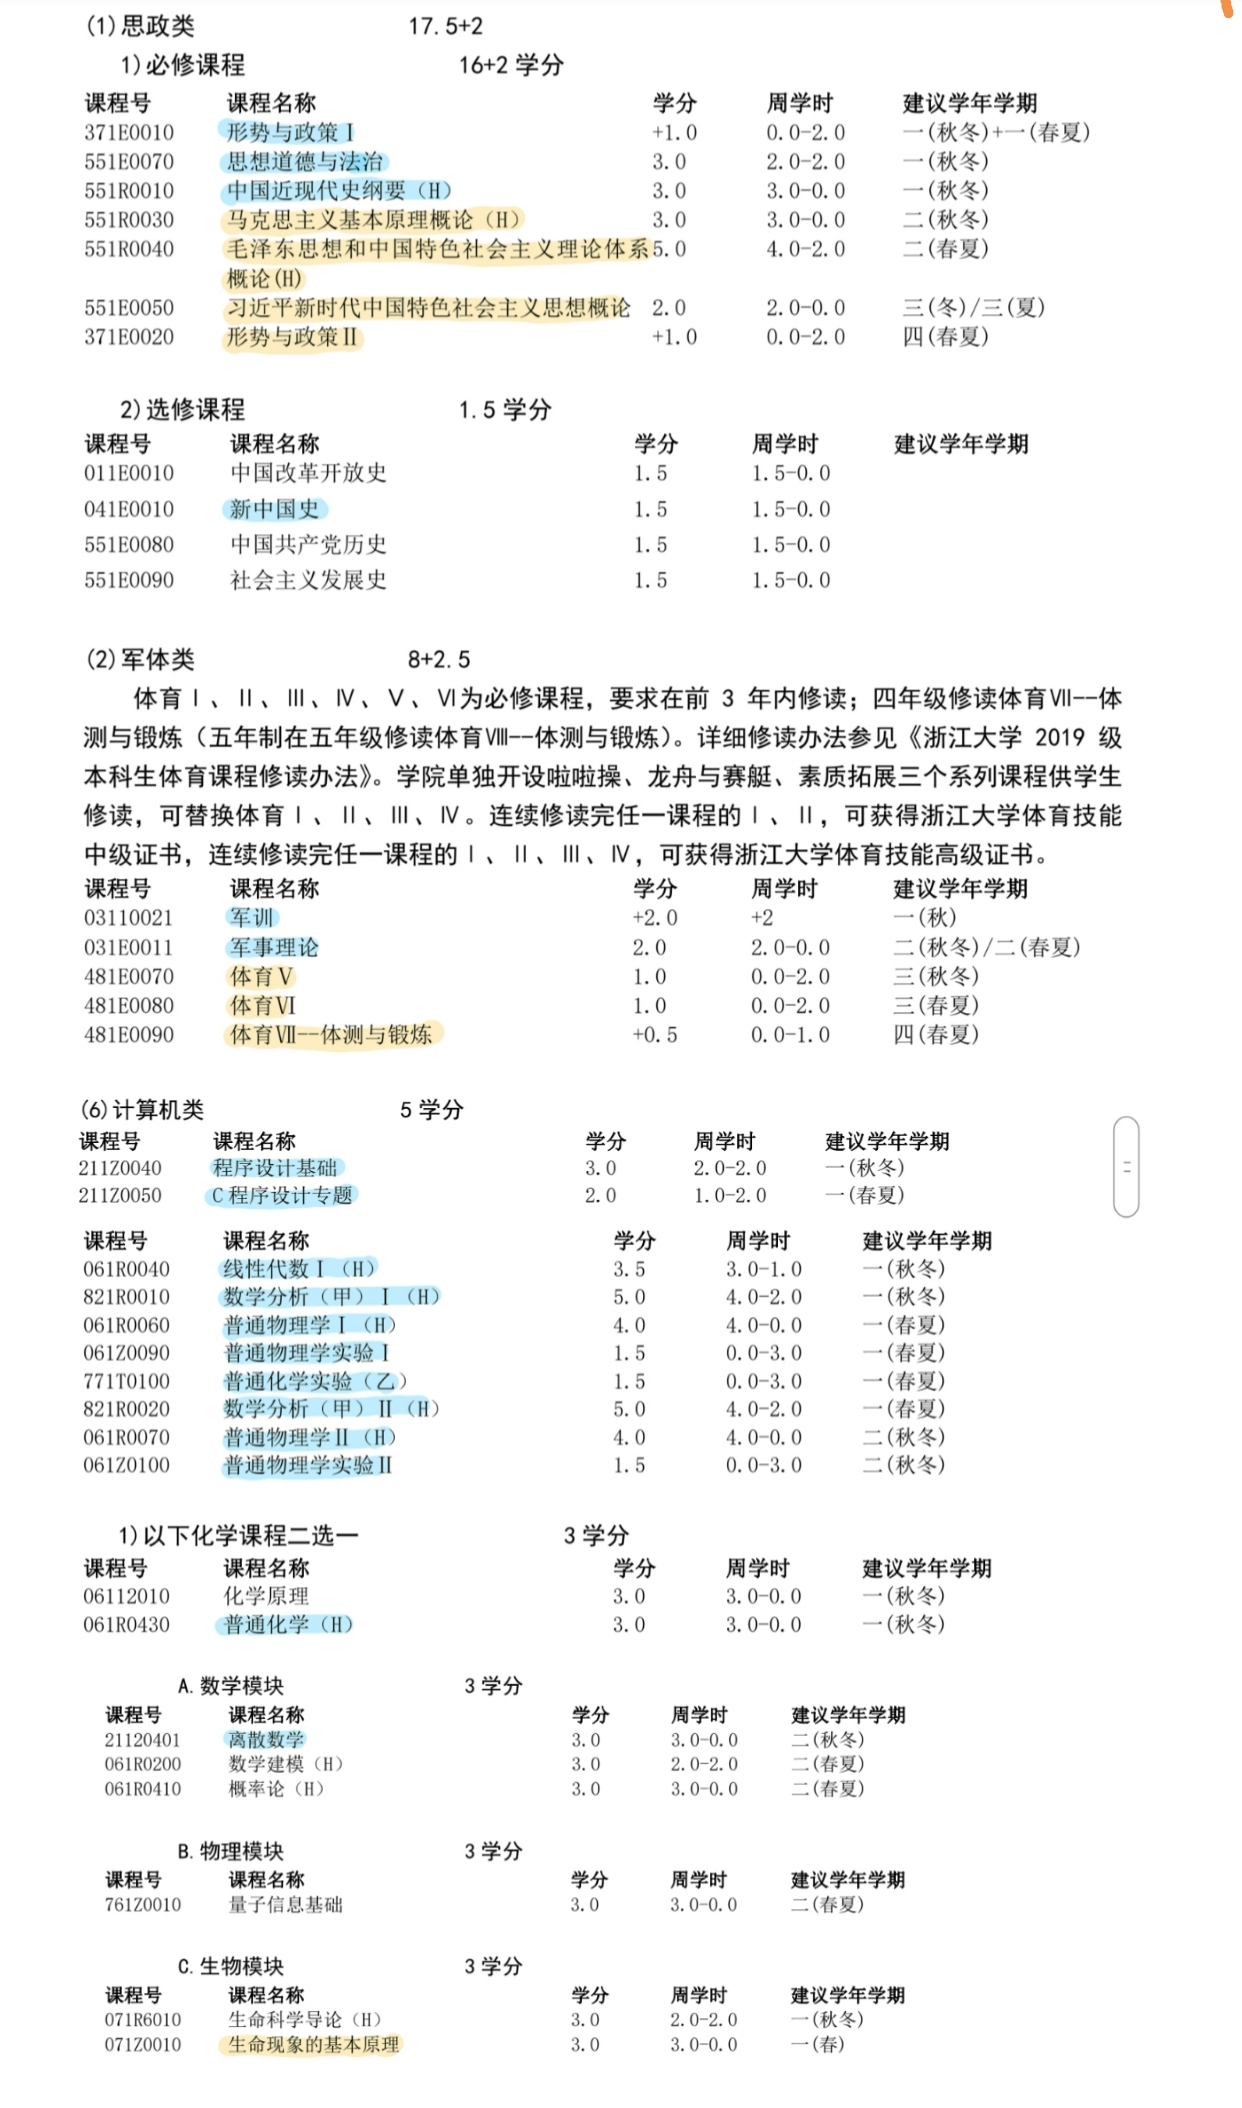
\includegraphics[width=1\textwidth]{1.jpg}
	\caption{\label{总结}课程汇总}
	\end{figure}

    \begin{figure}[H]
    \centering
    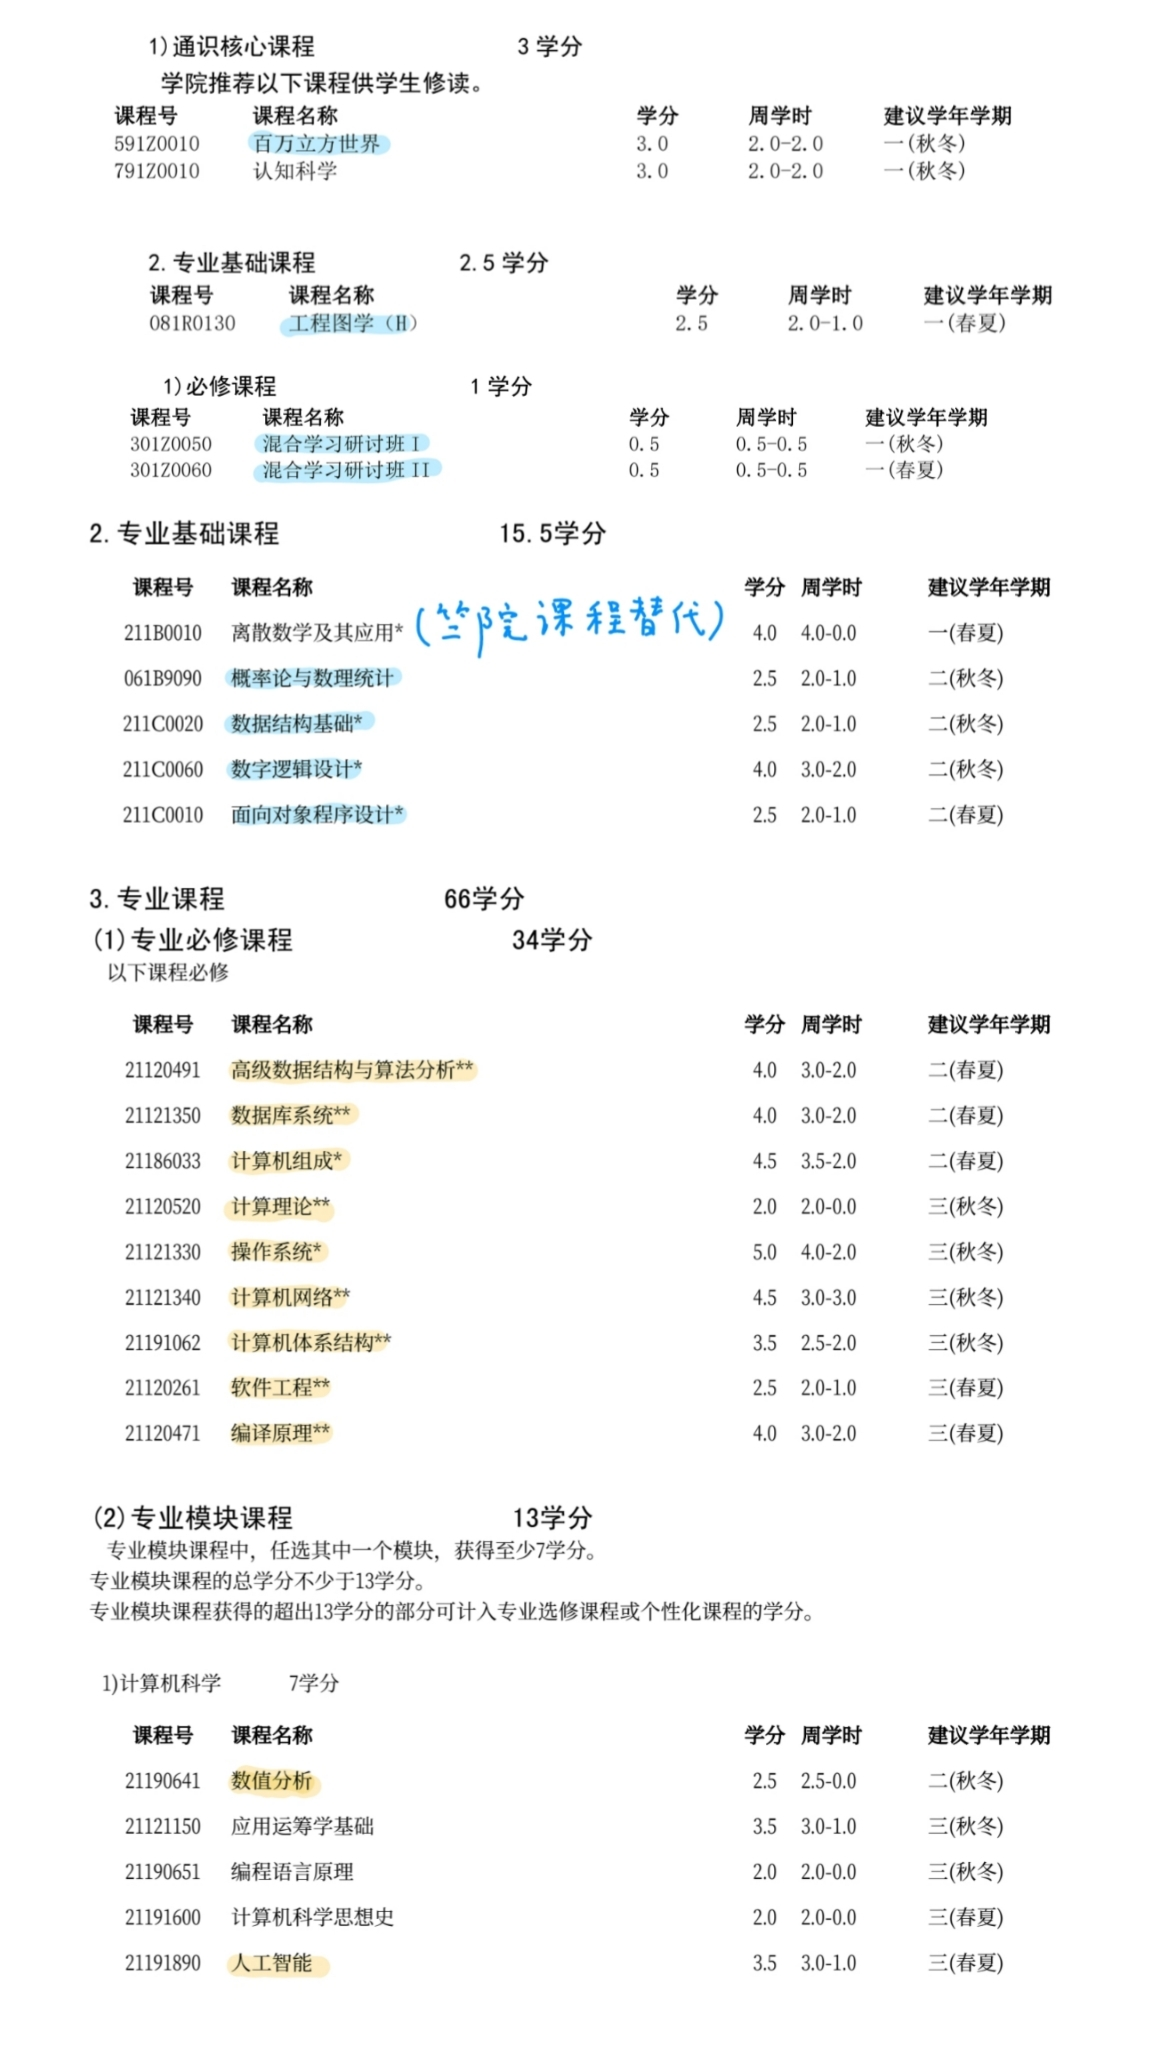
\includegraphics[width=1\textwidth]{2.jpg}
    \caption{\label{总结}课程汇总}
    \end{figure}

    \begin{figure}[H]
    \centering
    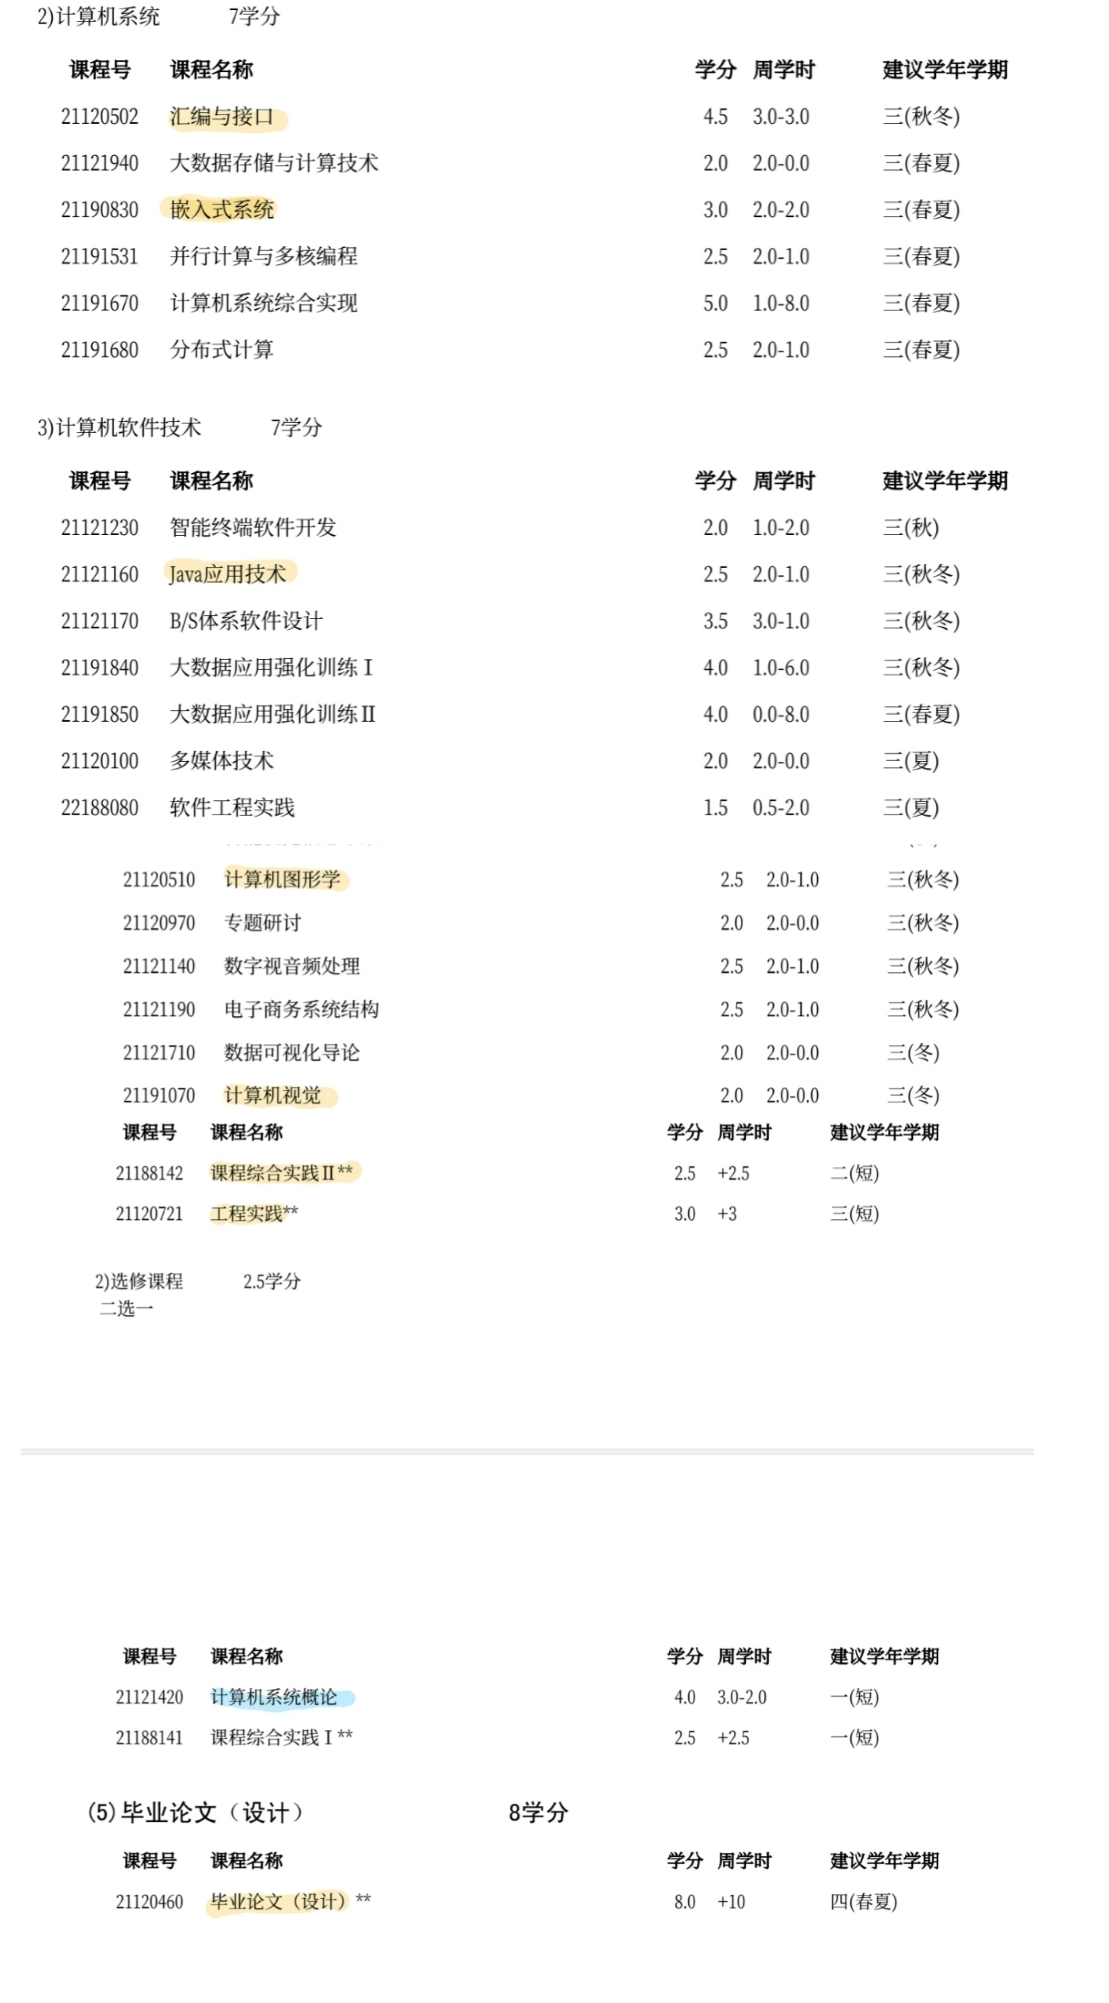
\includegraphics[width=1\textwidth]{3.jpg}
    \caption{\label{总结}课程汇总}
    \end{figure}

我目前在竺可桢学院混合班就读,目前为大二年级.主修专业是计算机科学与技术,以上培养方案中涂有蓝色的是我已经上完或正在上的课程,涂有黄色的是我计划未来要上的课程.

\section*{二:个人成绩汇总}

\subsection*{主修课程成绩}
主修专业平均绩点:4.37
    \begin{figure}[H]
    \centering
    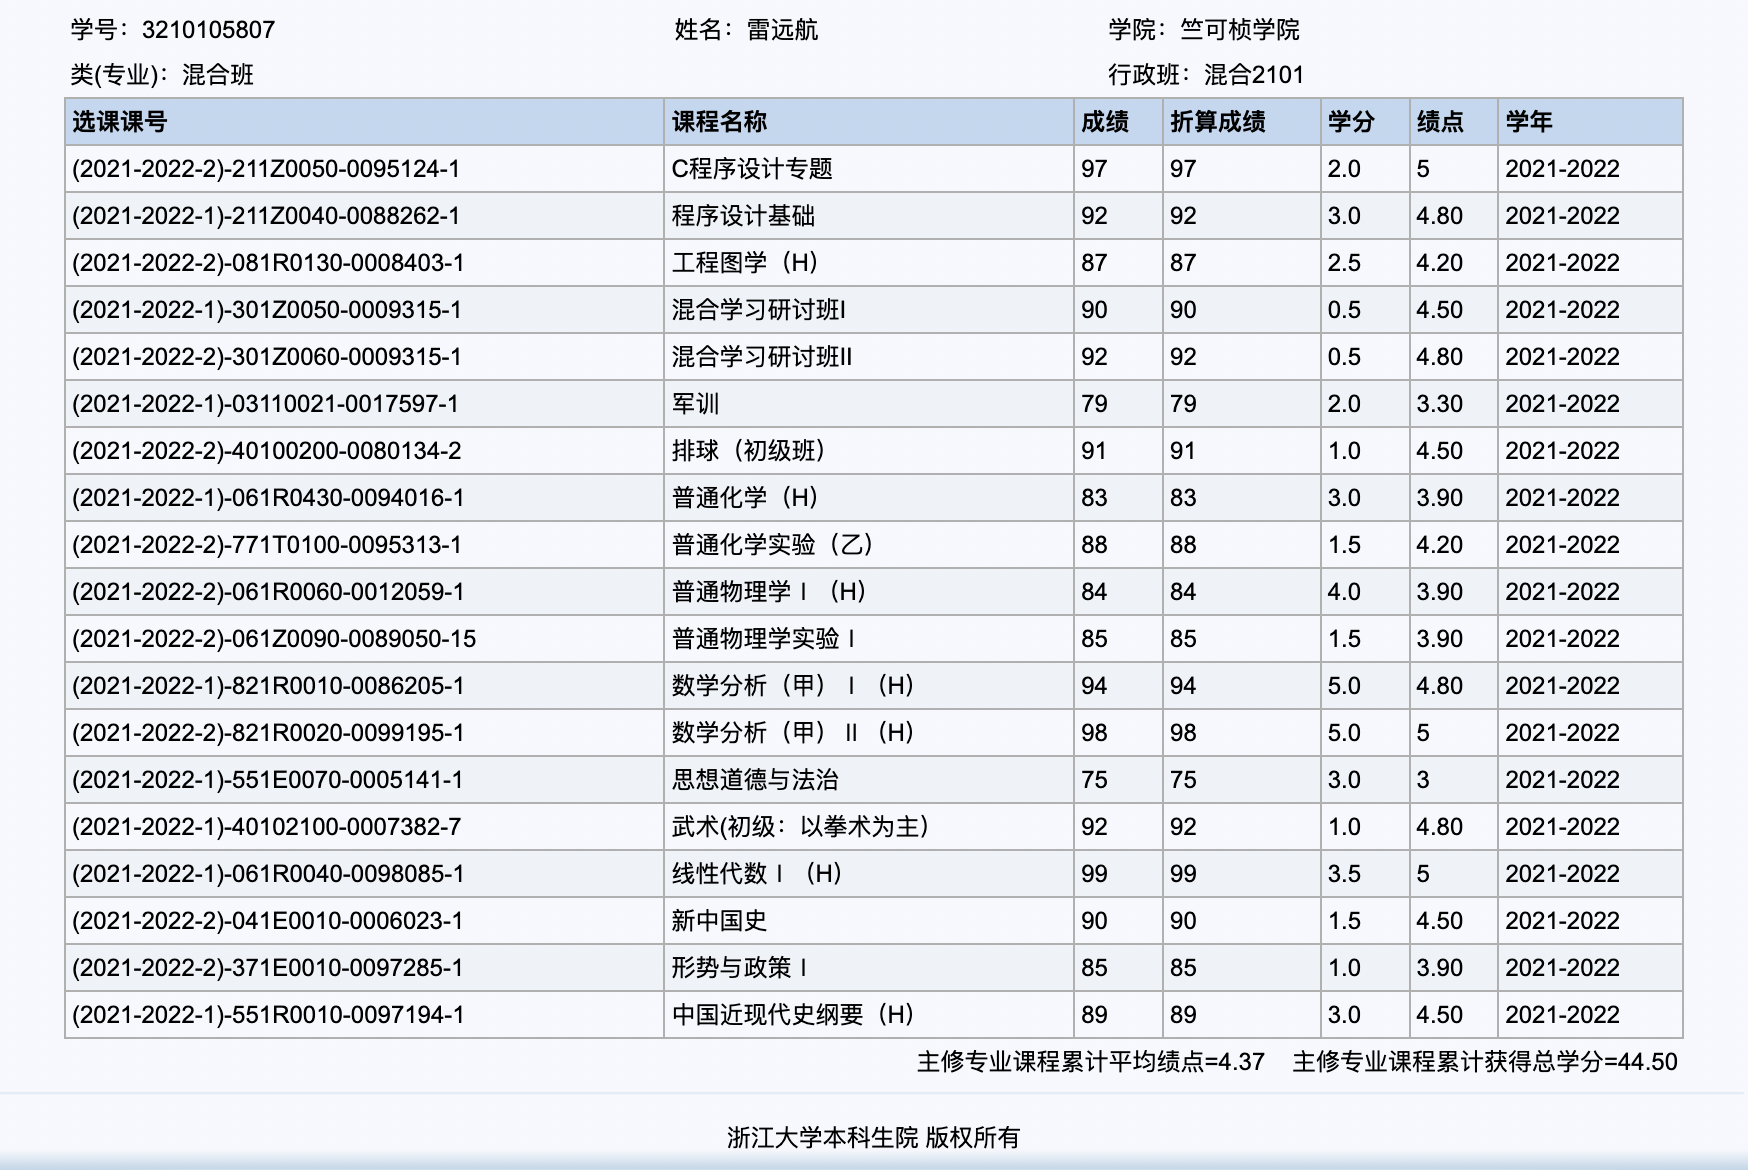
\includegraphics[width=1\textwidth]{4.png}
    \caption{\label{总结}成绩单}
    \end{figure}

\subsection*{全部课程汇总}
    \begin{figure}[H]
    \centering
    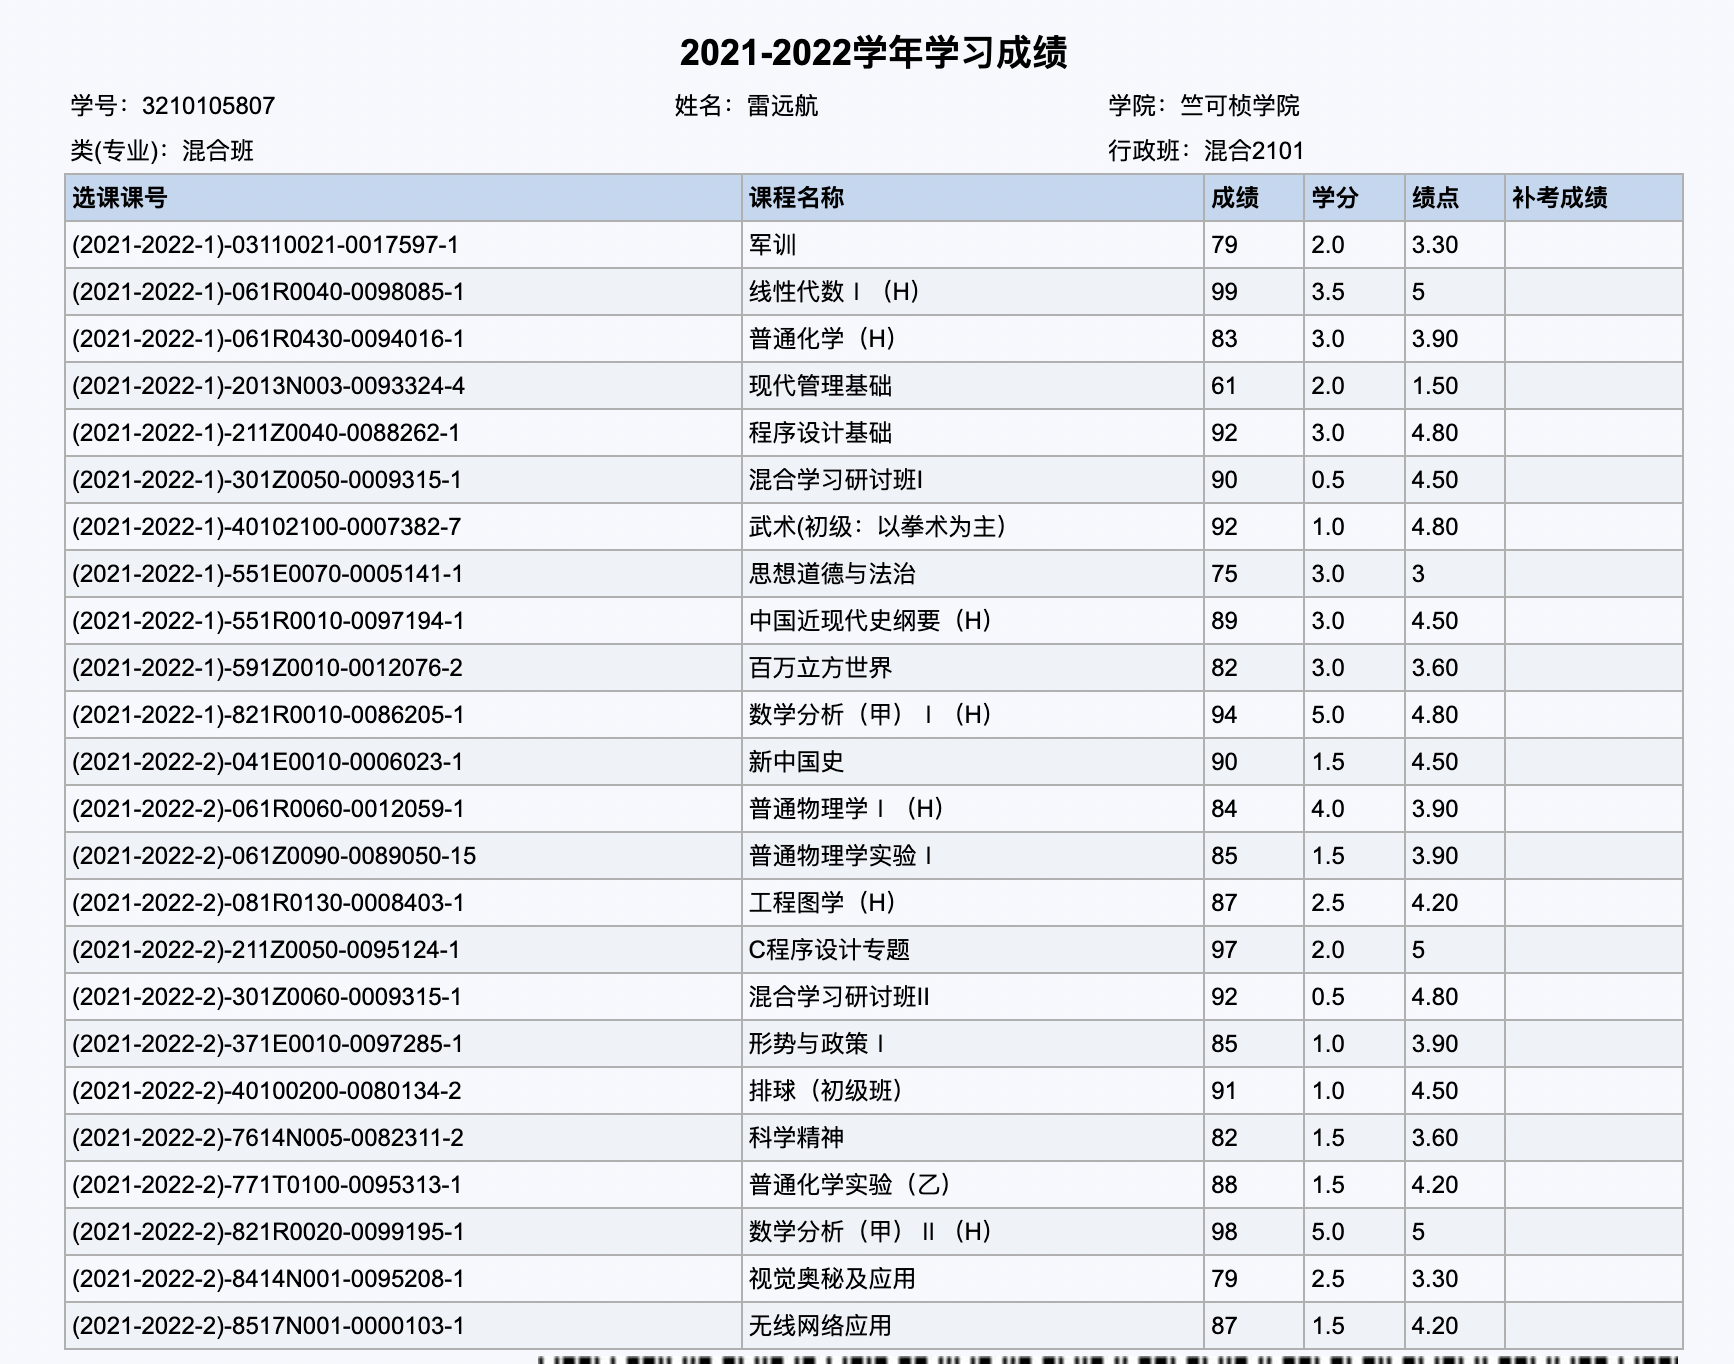
\includegraphics[width=1\textwidth]{5.png}
    \caption{\label{总结}成绩单}
    \end{figure}

    \begin{figure}[H]
    \centering
    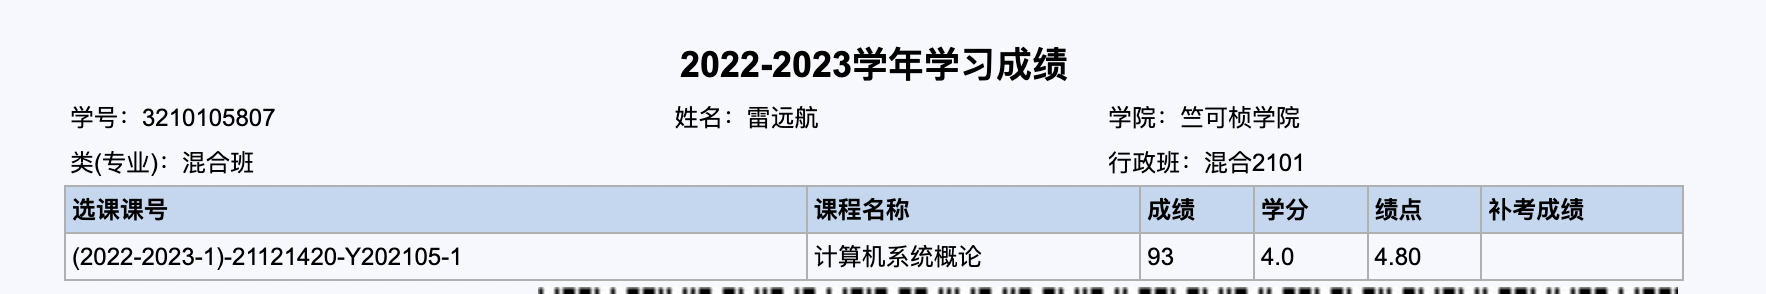
\includegraphics[width=1\textwidth]{6.png}
    \caption{\label{总结}成绩单}
    \end{figure}

\subsection*{与计算机相关的课程成绩}
程序设计基础:4.8

C程序设计专题:5.0

计算机系统概论:4.8

\subsection*{数学课程成绩}

数学分析1:4.8

数学分析2:5.0

线性代数:5.0

\section*{三:本学期课程安排}
    \begin{figure}[H]
    \centering
    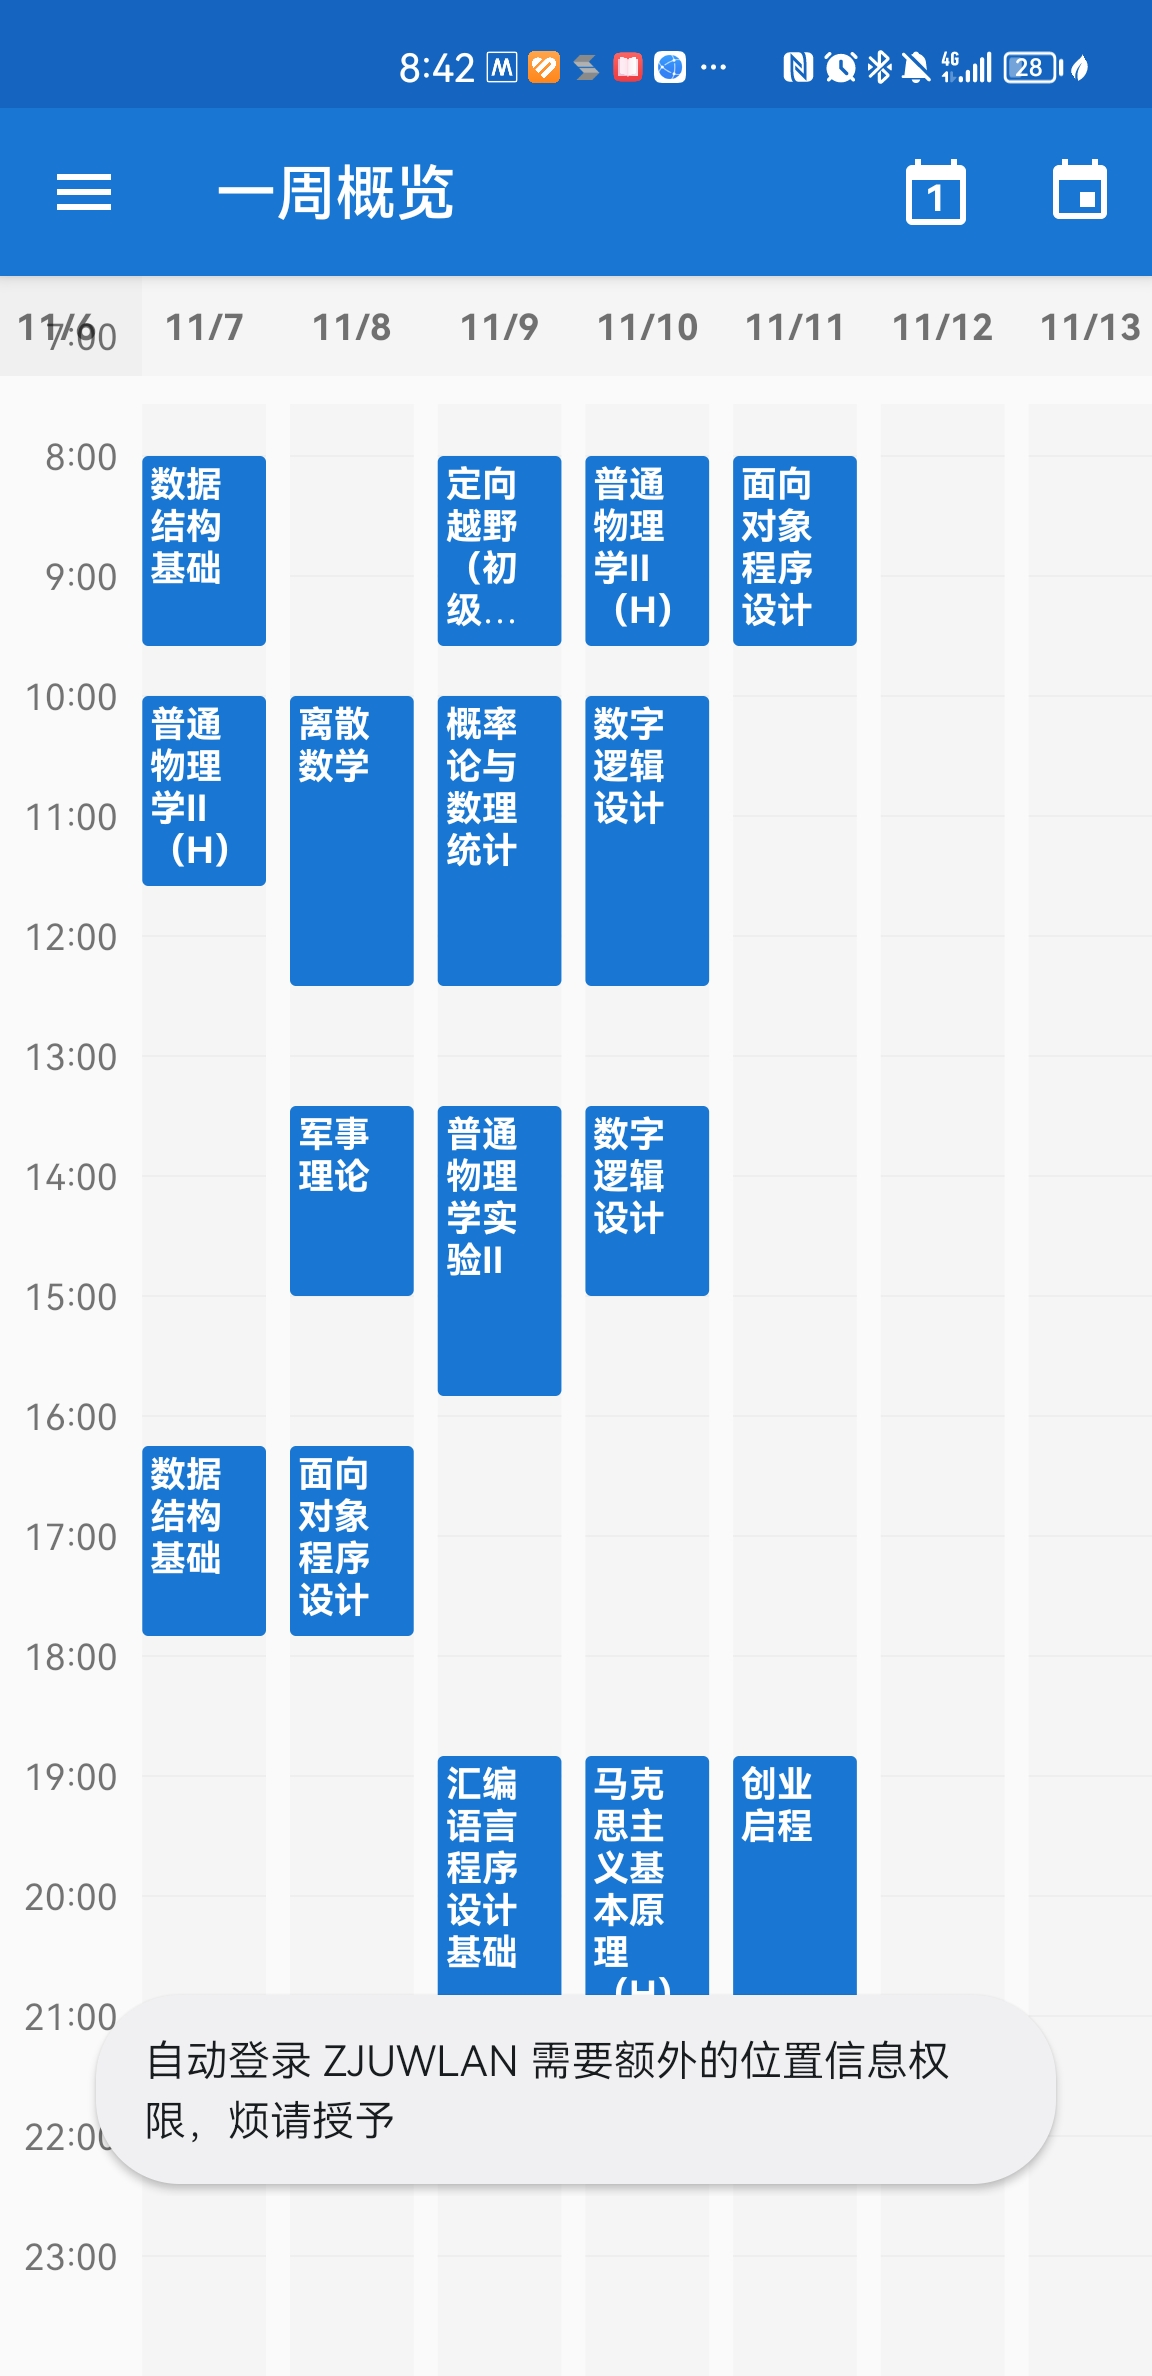
\includegraphics[width=0.5\textwidth]{7.jpg}
    \caption{\label{总结}成绩单}
    \end{figure}


\section*{四:我所具备的能力}

1.具有较好的C语言编程能力,在大一的C语言课上都取得不错的成绩(C小程4.8,C大程5.0).

2.熟悉C++语言编程,会使用STL,模版等重点内容,有一定的C++面向对象程序设计的能力,本学期正在进行"面向对象程序设计"的课程学习,并且自己的暑期已经自学完成一遍.

3.自学了python和Java的一些内容,对python的一些程序包有一定的了解(如:numpy,matplotlib等),了解Java一些的面向对象程序设计,可以看懂并写一些python和Java的代码.

4.会使用Linux,对shell编程,文件批处理,多文件编程,Makefile等有一定的了解,日常的程序书写和使用VsCode都采用命令行编译的方式,我有MacOS系统和Windows系统的两台笔记本,对适用于两个操作系统的任务都可以完成.


5.会使用git进行版本控制.

6.有一定的数据结构基础,本学期正在上数据结构的课程,并且自己也在假期自学过一些数据结构的基本内容.

7.会使用Markdown 和 Latex.

8.具有x86汇编语言的基础,本学期正在上相关的课程.

9.有较好的数学基础,在所上过的数学课程中都取得了较为不错的成绩.(数分1:4.8,数分2:5.0,线代:5.0)

10.正在学习图形学的入门课程,希望未来能进行一些图形学方面的研究和学习.
\section*{五:个人未来的展望}
学好自己的专业课程,在课程上能取得较好的成绩,掌握更多的技能和知识.同时本科阶段首先形成自己的科研的初步认识,学好自身专业课程的基础上,在自己的课程空余时间学习计算机图形学和计算机视觉的知识,并且使自己的数学基础能有进一步提升,同时也对计算机相关的领域都能有一定的了解和自己的看法,
在导师制的帮助下有一定科研方面的成长,感受科研的氛围,做一些自己能做的任务,并且在大四时能够有初步的提升.

本科毕业后希望能够在浙大的CAD\&CG实验室进行自己进一步的深造,此时自己具备的专业知识已经更加充足,希望能在自己的科研探索上有一定的成效.同时希望自己能够在高校进一步发挥自己的能力,丰富个人阅历,能在一些有水平的高校中从事自己的研究工作.





\end{document}
